\documentclass{beamer}
%
% Choose how your presentation looks.
%
% For more themes, color themes and font themes, see:
% http://deic.uab.es/~iblanes/beamer_gallery/index_by_theme.html
%
\mode<presentation>
{
  \usetheme{Madrid}      % or try Darmstadt, Madrid, Warsaw, ...
  \usecolortheme{default} % or try albatross, beaver, crane, ...
  \usefonttheme{default}  % or try serif, structurebold, ...
  \setbeamertemplate{navigation symbols}{}
  \setbeamertemplate{caption}[numbered]
}

\usepackage[spanish]{babel}
\usepackage[utf8x]{inputenc}
\usepackage{hyperref}

\hypersetup{
    colorlinks=true,       % false: boxed links; true: colored links
    linkcolor=white,          % color of internal links (change box color with linkbordercolor)
    citecolor=green,        % color of links to bibliography
    filecolor=magenta,      % color of file links
    urlcolor=cyan           % color of external links
}

\title[Taller ComCom de Git - Clase 1]{Taller ComCom de Git - Clase 1}
\author[Iván Arcuschin]{Iván Arcuschin Moreno}
\institute{ComCom - DC - FCEyN - UBA}
\date{11/03/2016}

% http://latexcolor.com/
\definecolor{lightseagreen}{rgb}{0.13, 0.7, 0.67}
\definecolor{tangelo}{rgb}{0.98, 0.3, 0.0}
\definecolor{git}{rgb}{0.94, 0.309, 0.2}

\setbeamercolor{structure}{fg=lightseagreen}

\newenvironment{ejercicio}[1]{
% \setbeamercolor{block title}{bg=tangelo, fg=white}
\begin{exampleblock}{#1}
}{
\end{exampleblock}
}

\newenvironment{resumen}[1]{
\setbeamercolor{block title}{bg=git, fg=white}
\begin{block}{#1}
}{
\end{block}
}

\newenvironment{comando}{
\setbeamercolor{block body}{bg=git, fg=white}
\begin{block}{}
\begin{center}
\LARGE
\begin{texttt}
}{
\end{texttt}
\end{center}
\end{block}
}

\begin{document}

\defverbatim{\gitstatusmodified}{
\begin{verbatim}
Untracked files:
README
nothing added to commit but untracked files present
\end{verbatim}
}

\defverbatim{\gitstatusready}{
\begin{verbatim}
Changes to be committed:
new file:   README
\end{verbatim}
}

\defverbatim{\gitstatusclean}{
\begin{verbatim}
nothing to commit, working directory clean
\end{verbatim}
}

\begin{frame}
  \titlepage
  \begin{figure}[ht]
      \begin{center}
          
\includegraphics[height=1in]{images/logo-taller.png}
      \end{center}
  \end{figure}
\end{frame}

\begin{frame}{Motivación 1/2}

    \begin{figure}[ht]
        \begin{center}
            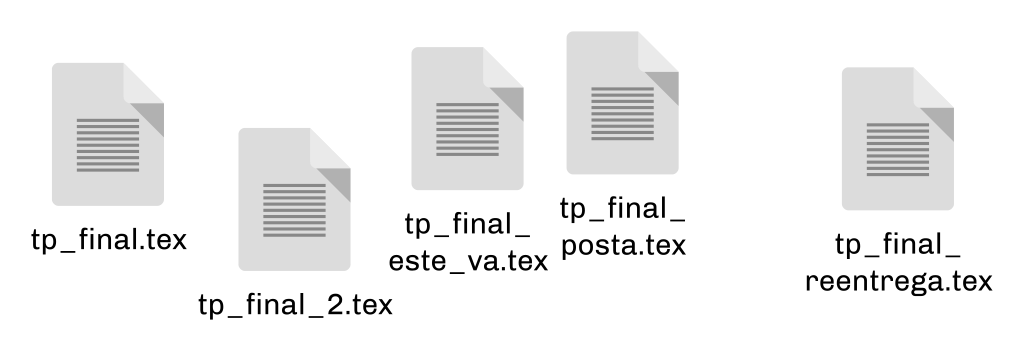
\includegraphics[height=1.5in]{images/caos.png}
        \end{center}
    \end{figure}

    \pause
    \begin{figure}[ht]
        \begin{center}
            
\includegraphics[height=1.5in]{images/horror.png}
        \end{center}
    \end{figure}

\end{frame}

\begin{frame}{Motivación 2/2}

    \begin{block}{Trabajando de a grupo}
        \begin{itemize}
            \item Enviar cambios por mail, o
            \pause
            \item Sincronizar cambios por Dropbox, o
            \pause
            \item Sincronizar cambios por Google Docs.
        \end{itemize}
    \end{block}

    \pause
    \begin{figure}[h]
        \begin{center}
            
\includegraphics[height=1.5in]{images/horror.png}
        \end{center}
    \end{figure}

\end{frame}

\begin{frame}{¿Qué es un Sistema de Control de Versiones?}

	\begin{block}{}
		Los Sistemas de Control de Versiones son una categoría de programas que permiten a un equipo manejar los cambios en el código fuente de un proyecto a lo largo del tiempo.

		Dichos programas llevan un seguimiento de las modificaciones que hacemos al código, y en caso de que nos equivoquemos en algo es posible volver a tras y comparar el código actual con otras versiones anteriores para ayudar a arreglar el error.

		También, permiten que varias personas distintas del equipo modifiquen el código a la vez y compartan los cambios, tratando que prevenir posibles conflictos, y en caso de que los hubiera ayudando a identificarlos y resolverlos.

	\end{block}

    \pause
    \begin{resumen}{Es decir..}
        \begin{itemize}
            \item Permiten arreglar \textit{accidentes} y volver a versiones anteriores del código.
            \item Permiten compartir código con otras personas.
        \end{itemize}
	\end{resumen}

\end{frame}

\begin{frame}{¿Qué es Git?}

	\begin{block}{}
		Git es un Sistema de Control de Versiones \textbf{distribuido y de código abierto}.
        Además fue diseñado con enfasis en la \textbf{performance} (para manejar proyectos muy grandes), \textbf{seguridad} y \textbf{flexibilidad}.
        Provee un amplio conjunto de comandos que permiten realizar operaciones de alto y bajo nivel.
	\end{block}

    \begin{figure}[ht]
        \begin{center}
            
\includegraphics[height=1.5in]{images/logo-git.png}
        \end{center}
    \end{figure}
\end{frame}

\begin{frame}[fragile]{Configuraciones iniciales}

	\begin{block}{Clave ssh}
		Para poder trabajar comodamente con repositorios Git que estén en internet (GitHub, Bitbucket, GitLab, etc) podemos configurar una clave ssh que nos identifique con el servidor que estemos usando.

        Por ejemplo, en GitLab:

        \url{http://doc.gitlab.com/ce/gitlab-basics/create-your-ssh-keys.html}
	\end{block}

    \begin{block}{Tu identidad}
        Es importante establecer nuestro nombre y email ya que estos van a ir asociados con los cambios que hagamos:

        \vspace{0.5em}

        \texttt{git config --global user.name "John Doe"}

        \texttt{git config --global user.email johndoe@example.com}
    \end{block}


\end{frame}

\begin{frame}[t]{Obteniendo un repositorio Git}
%    \begin{block}{Inicializando un repositorio en un directorio existente}
%        Para crear un nuevo repositorio local podemos ir al directorio y ejecutar
%        \texttt{git init}. Esto crea un subdirectorio \textit{.git} que tiene todos
%        los archivos necesarios del repositorio.
%    \end{block}

%    \begin{block}{Clonando un repositorio existente}
    \begin{comando}
        git clone
    \end{comando}

    \pause
	\begin{block}{}
        Para obtener una copia local de un repositorio existente en algún servidor,
        utilizamos el comando \texttt{git clone [URL]} (sin los corchetes)
    \end{block}

    \pause
    \vspace{1em}
    \begin{ejercicio}{Ejercicio}
        \textit{Clonar} el repositorio que tiene URL: \textbf{git@gitlab.com:talleres-comcom/taller-git.git}

        \vspace{0.5em}
        Es un repositorio que tiene los fuentes\ \LaTeX\ de estas diapositivas !
    \end{ejercicio}
\end{frame}

\begin{frame}[t]{Preparando cambios}

    \begin{comando}
        git add
    \end{comando}

    \pause
    \begin{block}{Es corta la bocha}
        \begin{enumerate}
            \item Creamos/Modificamos el archivo en cuestión.
            \item Ejecutamos \texttt{git add [nombre del archivo]}
        \end{enumerate}
    \end{block}

    \pause
    \vspace{1em}
    \begin{ejercicio}{Ejercicio}
        Adentro del repositorio que \textit{clonaron} recién, crear un archivo y
        marcarlo como \textit{preparado} usando el comando \texttt{git add}.
    \end{ejercicio}

\end{frame}

\begin{frame}[t]{Confirmando cambios}

    \begin{comando}
        git commit
    \end{comando}

    \pause
    \begin{block}{Es corta la bocha}
        \begin{enumerate}
            \item Ejecutamos \texttt{git commit}
            \item Nos va a saltar un editor de texto para que le pongamos un \textbf{mensaje a los cambios}.
            \item Guardamos el mensaje, y listo.
        \end{enumerate}
    \end{block}

    \pause
    \vspace{1em}
    \begin{ejercicio}{Ejercicio}
        Confirmar los cambios que \textit{prepararon} en la diapo anterior.
    \end{ejercicio}

\end{frame}

\begin{frame}[fragile, t]{¿Está preparado, confirmado o ninguna de las dos?}

    \begin{comando}
        git status
    \end{comando}

    \begin{block}{No es lo mismo!}
        Las modificaciones que hacemos pueden estar en \textbf{3 estados} distintos:
        \begin{itemize}
            \pause
            \item<2-> \textbf{Modificado (modified)}: las modificaciones todavía no están \textit{preparadas o listas}.
            \item<3-> \textbf{Preparado (staged)}: las modificaciones están marcadas como \textit{preparadas o listas} e
                irán en la proxima \textit{confirmación de cambios}.
            \item<4-> \textbf{Confirmado (committed)}: las modifiaciones están guardadas con un \textit{mensaje} que explica los cambios realizados.
        \end{itemize}
    \end{block}

    \only<2> {
        \gitstatusmodified
    }
    \only<3> {
        \gitstatusready
    }
    \only<4> {
        \gitstatusclean
    }

\end{frame}

\begin{frame}[fragile]{Viendo los cambios preparados}
    Muchas veces es conveniente ver cuales son los cambios realizados antes de mandarlos a Preparado.
    Para esto tenemos el comando \texttt{git diff}, que muestra las diferencias entre lo que hay en
    tu directorio de trabajo con lo que hay en tu área de preparación.

    \vspace{1em}

    Si en cambio, queremos ver los cambios que preparamos y que irán en la próxima confirmación, podemos usar \texttt{git diff --staged}.

\end{frame}

\begin{frame}{Confirmando (``commiteando'') cambios}
    Una vez que tenemos nuestros cambios listos en el area de preparación, podemos
    utilizar el comando \texttt{git commit} para confirmarlos. Ningún cambio o archivo
    que no esté en el area de preparación se incluirá en la confirmación.

    \vspace{1em}

    Cada confirmación requiere de un mensaje con una descripción de los cambios realizados.
    Por ejemplo: \texttt{git commit -m ``Agrego archivo README''}. Si ejecutamos
    \texttt{git commit} sin el parámetro \texttt{-m}, se nos abrirá el editor de texto configurado para Git,
    en el que podremos escribir una descripción de forma más cómoda.

\end{frame}

\begin{frame}{Viendo la historia de los commits}

    Después de haber hecho varios \textit{commits}, o si acabamos de clonar un repositorio
    de internet, puede que querramos ver el historial de commits para ver cuales
    fueron las modificaciones que se hicieron. Esto se puede lograr utilizando el
    comando \texttt{git log}.

\end{frame}

\begin{frame}[fragile]{Trabajando con repositorios remotos}

    Los repositorios remotos son versiones de tu proyecto que se encuentran alojados
    en Internet o en algún punto de la red. Puedes tener varios, cada uno de los cuales
    puede ser de sólo lectura, o de lectura/escritura, según los permisos que tengas.

    \vspace{0.5em}

    Colaborar con otros implica gestionar estos repositorios remotos, y mandar (push) y recibir (pull)
    datos de ellos cuando necesites compartir cosas.

    \vspace{0.5em}

    Para ver qué repositorios remotos están configurados, podemos usar el comando \texttt{git remote}.
    Si acabamos de clonar el repositorio que tiene los fuentes de estas diapositivas y corremos \texttt{git remote -v}, veremos:
    \begin{verbatim}
origin  git@github.com:FlyingPumba/git-intro.git (fetch)
origin  git@github.com:FlyingPumba/git-intro.git (push)
    \end{verbatim}

    Y si tenemos un repositorio creado localmente y queremos añadir un remoto, usamos \texttt{git remote add [nombre] [url]}.

\end{frame}

\begin{frame}{Ramificaciones en Git}

    Cada vez que realizamos una confirmación (commit), Git almacena entre otras cosas uno o varios punteros a las confirmaciones que
    sean padres directos de esta.

    Una rama o branch en Git no es más que un puntero especial parado en un commit. Ejecutar \texttt{git branch} nos mostrará las ramas actuales. Veamos un ejemplo sencillo:

    %\begin{columns}
    %    \column{0.5\textwidth}
    %    \begin{figure}[ht]
    %        \begin{center}
    %            \includegraphics[height=1.1in]{images/branch-and-history.png}
    %        \end{center}
    %        \caption{La rama ``master'' apunta al commit \textit{f30ab}}
    %    \end{figure}
    %    \column{0.5\textwidth}
    %    \begin{figure}[ht]
    %        \begin{center}
    %            \includegraphics[height=1.1in]{images/head-to-master.png}
    %        \end{center}
    %        \caption{Creamos una nueva rama ejecutando \texttt{git branch testing}}
    %    \end{figure}
    %\end{columns}

\end{frame}

\begin{frame}{Cambiando de rama}

    %\begin{figure}[ht]
    %    \begin{center}
    %        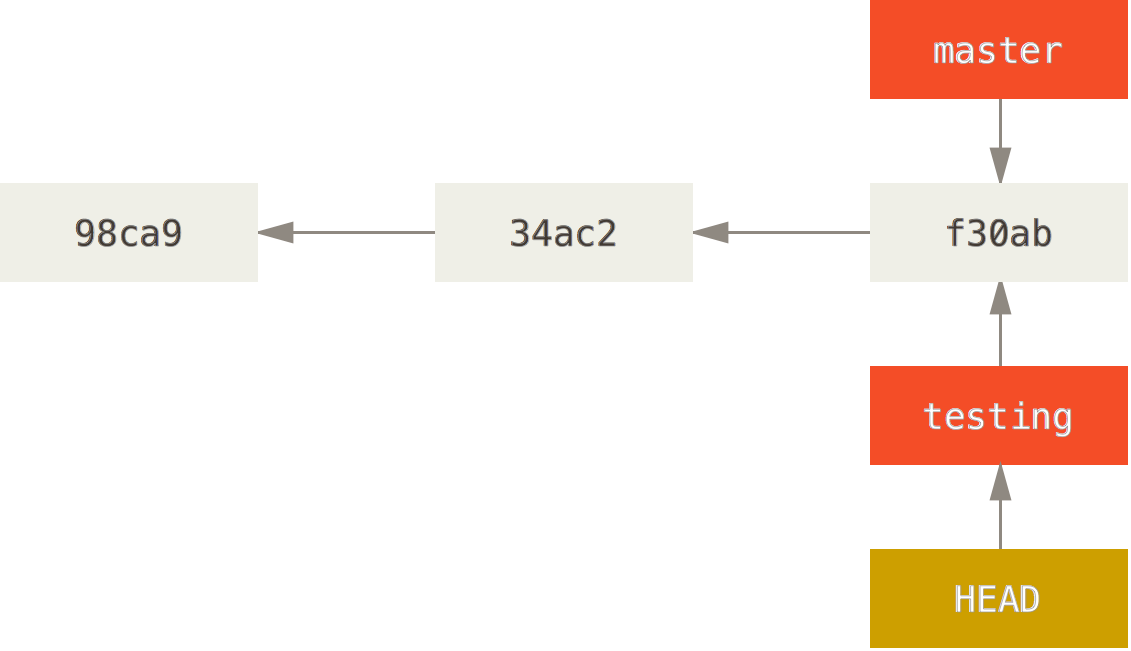
\includegraphics[height=1in]{images/head-to-testing.png}
    %    \end{center}
    %    \caption{Si queremos cambiar de rama, podemos ejecutar \texttt{git checkout testing}}
    %\end{figure}
    %\begin{figure}[ht]
    %    \begin{center}
    %        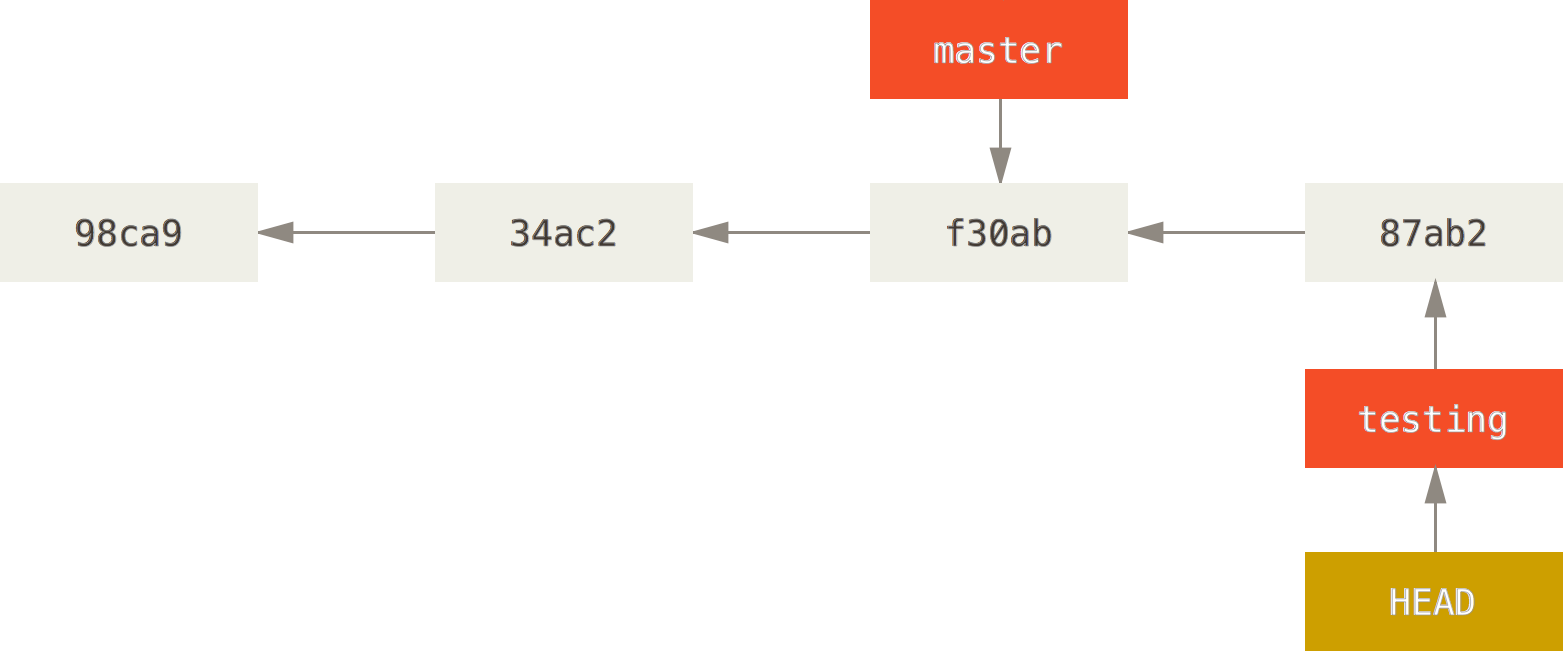
\includegraphics[height=1in]{images/advance-testing.png}
    %    \end{center}
    %    \caption{Y los siguientes commits serán agregados a la rama ``testing''}
    %\end{figure}

\end{frame}

\begin{frame}{Ramas remotas}

    Ademas de tener ramas locales, podemos tenemos ramas remotas, que referencian al estado de ramas en tus repositorios remotos.
    Si por ejemplo quisieramos saltar a la rama ``master'' en el repositorio remoto ``origin'' podríamos utilizar el comando \texttt{git checkout origin/master}.

    \vspace{1em}

    Nuestras ramas locales no sincronizan automaticamente con los repositorios remotos. Por esta razón, si tenemos una rama llamada ``master'' de forma local que
    apunta a la rama remota ``origin/master'' podemos actualizarla parandonos en ``master'' y ejecutando \texttt{git pull origin master}.

    \vspace{1em}

    De forma análoga, si queremos publicar cambios locales aun repositorio remoto, tenemos el comando \texttt{git push}. Si estamos parados en la rama ``master'':
    \texttt{git push origin master}.

\end{frame}

\begin{frame}{Fusionando ramas}

    Supongamos que tenemos una rama ``iss53'' en la cual hemos terminado de arreglar un error, y queremos combinarla con la rama ``master''.
    Para ello, simplemente nos paramos en ``master'' (\texttt{git checkout master}) y ejecutamos: \texttt{git merge iss53}.

	%\begin{figure}[ht]
	%	\begin{center}
	%		\includegraphics[height=1.5in]{images/basic-merging-1.png}
	%	\end{center}
	%	\caption{Antes del merge}
	%\end{figure}

\end{frame}

\begin{frame}{Fusionando ramas}

    Supongamos que tenemos una rama ``iss53'' en la cual hemos terminado de arreglar un error, y queremos combinarla con la rama ``master''.
    Para ello, simplemente nos paramos en ``master'' (\texttt{git checkout master}) y ejecutamos: \texttt{git merge iss53}.

	%\begin{figure}[ht]
	%	\begin{center}
	%		\includegraphics[height=1.5in]{images/basic-merging-2.png}
	%	\end{center}
	%	\caption{Después del merge}
	%\end{figure}

\end{frame}

\begin{frame}{Otros comandos útiles}

    \begin{itemize}
        \item \texttt{git fetch [remote repository]}: para traer todos los datos de un repositorio remoto.
        \item \texttt{git reset}: para deshacer cambios, ya sea en el area de trabajo o en los commits.
        \item \texttt{git rm}: para borrar un archivo y pasarlo al area de preparación.
        \item \texttt{git mv}: para mover/renombrar un archivo y pasarlo al area de preparación.
        \item \texttt{git show}: muestra información de distintos objectos de Git: commits, tags, etc.
        \item \texttt{git stash}: guarda el estado del area de trabajo y lo limpia.
        \item \texttt{git rebase [branch]}: aplica todos los commits que difieren entre un branch y el que estamos parados.
        \item \texttt{git tag [etiqueta] [commit hash]}: ponerle una etiqueta a un commit.
    \end{itemize}

\end{frame}

\begin{frame}{Bibliografía extra}

    \begin{itemize}
        \item Git Community book, disponible online y en español: \url{https://git-scm.com/book/es/v2}
		\item \texttt{git help [command]} para ver la documentación de cualquier comando de Git.
		\item A visual Git reference: \url{http://marklodato.github.io/visual-git-guide/index-es.html}
		\item Try Git online: \url{https://try.github.io}
        \item Git - SVN Crash Course: \url{https://git-scm.com/course/svn.html}
    \end{itemize}

\end{frame}

\begin{frame}{Mini ejercicio de práctica}

	\begin{block}{Básico}
		\begin{enumerate}
			\item Instalar Git en tu máquina.
			\item Clonar el repositorio que tiene los fuentes de estas diapositivas. (git@github.com:FlyingPumba/git-intro.git)
			\item Abrir el archivo \textit{main.tex} y \textbf{arregkar} el typo en esta oración.
			\item Pasar \textit{main.tex} al area de preparados.
			\item Confirmar los cambios.
		\end{enumerate}
	\end{block}

\end{frame}


\begin{frame}{Mini ejercicio de práctica}

	\begin{block}{Avanzado}
		\begin{enumerate}
			\item Crearse una cuenta en \url{GitHub.com}
			\item Ir a la página del repositorio que tiene los fuentes de estas diapositivas \url{https://github.com/FlyingPumba/git-intro} y \textit{forkear} el proyecto a un repositorio personal en GitHub.
			\item Agregar a su repositorio local un nuevo remoto llamado ``fork'' que apunte a su repositorio remoto en GitHub.
			\item Pushear la rama ``master'' al repositorio remoto ``fork''.
			\item Hacer un \textit{Pull request} en GitHub.
		\end{enumerate}
	\end{block}

\end{frame}

\end{document}
